\section{theorem13}
\begin{theorem}
\end{theorem}

Suppose we have the following local diagram and a sheaf on it :

\begin{figure}[H] % Optional: [h] means here, [t] for top, [b] for bottom, [p] for page of floats
    \centering
    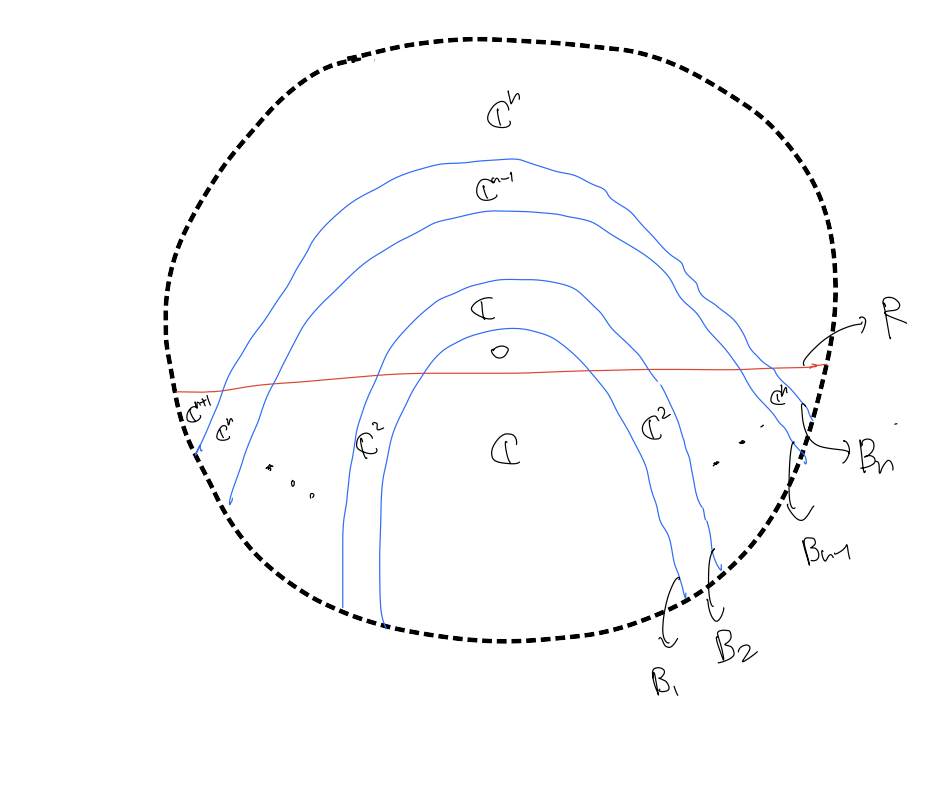
\includegraphics[width=\linewidth]{diagrams/theorem13/1.png} % Adjust the width as needed
    \caption{Your caption here}
    \label{fig:your-label}
\end{figure}

If we iteratively appy reverse Reidemeister \RN{2} $n$ times(in the $i^{th}$ iteration we apply reverse Redemeister \RN{2} to $B_i$ and $R$), we get the following diagram and a sheaf :

\begin{figure}[H] % Optional: [h] means here, [t] for top, [b] for bottom, [p] for page of floats
    \centering
    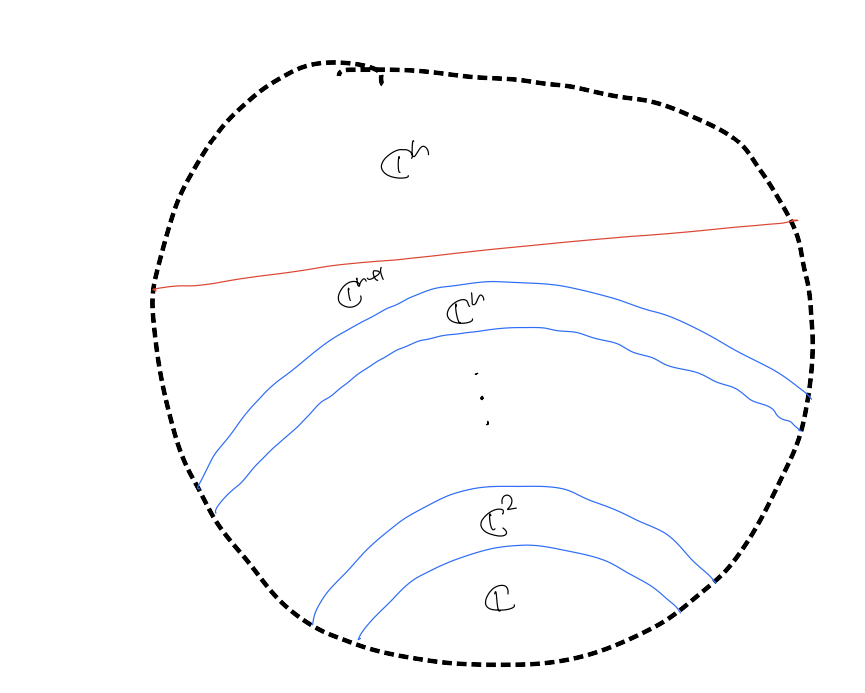
\includegraphics[width=\linewidth]{diagrams/theorem13/2.png} % Adjust the width as needed
    \caption{Your caption here}
    \label{fig:your-label}
\end{figure}
(proof) If $n=1$, then this is just a single reverse Reidemeister \RN{2} move. If $n>1$, then by the induction hypothesis, after applying $n-1$ reverse Reidemeister \RN{2} moves, we get :

\begin{figure}[H] % Optional: [h] means here, [t] for top, [b] for bottom, [p] for page of floats
    \centering
    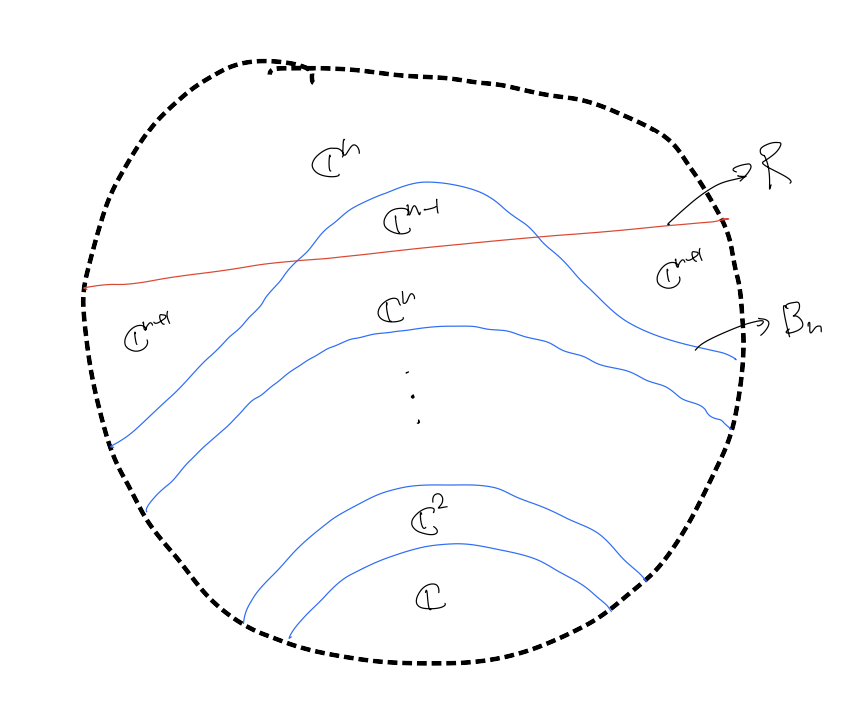
\includegraphics[width=\linewidth]{diagrams/theorem13/3.png} % Adjust the width as needed
    \caption{Your caption here}
    \label{fig:your-label}
\end{figure}

To the above diagram and the sheaf, we apply reverse Reidemeister \RN{2}(on $R$ and $B_n$), we get the final diagram:

\begin{figure}[H] % Optional: [h] means here, [t] for top, [b] for bottom, [p] for page of floats
    \centering
    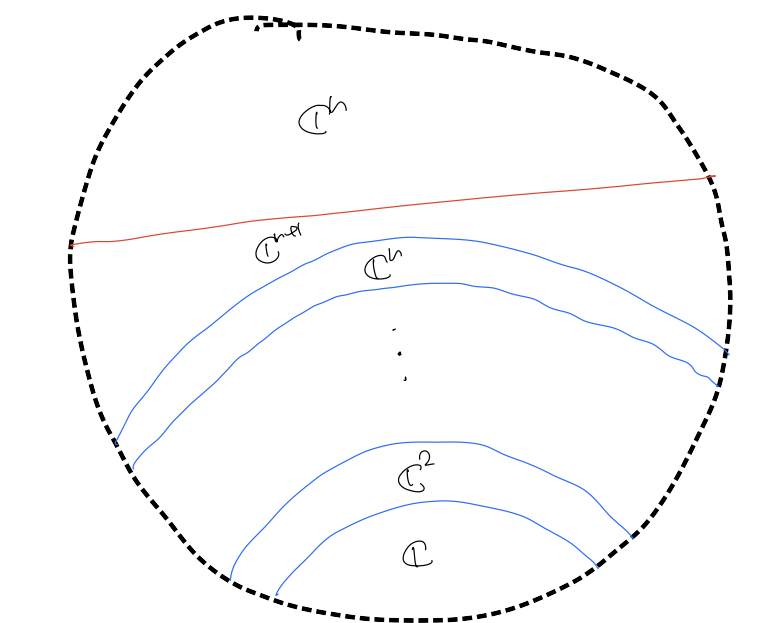
\includegraphics[width=\linewidth]{diagrams/theorem13/4.png} % Adjust the width as needed
    \caption{Your caption here}
    \label{fig:your-label}
\end{figure}